\section{Predicting Both Teams' Scores}\label{sec:scoremodel}

\subsection{Why two scores}

The object the engine needs is the joint distribution over $(h,a)$. Predicting each team's score is the natural first step: the two predictions locate the centre of that distribution and the spread of the residuals around them gives its width. A model for the margin alone discards the level of scoring; a 30--27 game and a 17--14 game have the same margin and very different distributions of totals and of every strike.

\subsection{Models and evaluation}

Table~\ref{tab:models} lists the models. All use the 759 non-market features of Section~\ref{sec:data}; the closing line is a benchmark only. Evaluation is walk-forward: train on every season before $t$, test on season $t$, for $t = 2010,\dots,2025$ (4,363 test games).

\begin{table}[H]
\centering
\small
\begin{tabular}{p{3.6cm}p{6.2cm}p{4cm}}
\toprule
\textbf{Model} & \textbf{Inputs} & \textbf{Role} \\
\midrule
League average & Mean scores in the training seasons & Floor \\
Elo & Results only; implied spread is Elo difference / 25 & Rating baseline \\
Two-output ridge regression & 759 features, median-imputed, standardised, penalty by cross-validation & Linear baseline \\
Two-output random forest & 759 features, 500 trees, at least 20 games per leaf, 30\% of features per split, no tuning & Main model: predicts $(h,a)$ jointly \\
Closing line & Consensus sportsbook spread and total & Benchmark \\
\bottomrule
\end{tabular}
\caption{Models compared. The forest predicts the two scores as a pair: each leaf holds the mean home and away score of similar past games.}
\label{tab:models}
\end{table}

\subsection{Point accuracy}

\begin{table}[H]
\centering
\small
\begin{tabular}{lcccc}
\toprule
\textbf{Model} & \textbf{Home score} & \textbf{Away score} & \textbf{Margin} & \textbf{Total} \\
\midrule
League average & 8.09 & 7.91 & 11.18 & 11.02 \\
Elo & -- & -- & 10.38 & -- \\
Two-output ridge & 7.62 & 7.40 & 10.34 & 10.63 \\
Two-output random forest & 7.63 & 7.45 & 10.35 & 10.66 \\
Closing line & -- & -- & \textbf{10.05} & \textbf{10.47} \\
\bottomrule
\end{tabular}
\caption{Mean absolute error in points, walk-forward 2010--2025.}
\label{tab:mae}
\end{table}

The forest explains 10.8\% of the variance of the home score and 9.3\% of the away score out of sample. These numbers are normal for the problem: a single game is mostly noise around a modest signal, and the closing line, with every input a bettor can find, explains only a little more. The forest and the ridge are indistinguishable at every target. On the margin they are 0.03--0.04 points better than Elo and 0.3 points worse than the line (Figure~\ref{fig:mae_season}); the line has the lowest error in 15 of 16 seasons. Straight-up winner accuracy is 64.7\% for the forest, 64.6\% for ridge, 64.5\% for Elo and 66.3\% for the line. Against the spread the forest picks the covering side 49.9\% of the time, as an efficient line implies.

\begin{figure}[H]
\centering
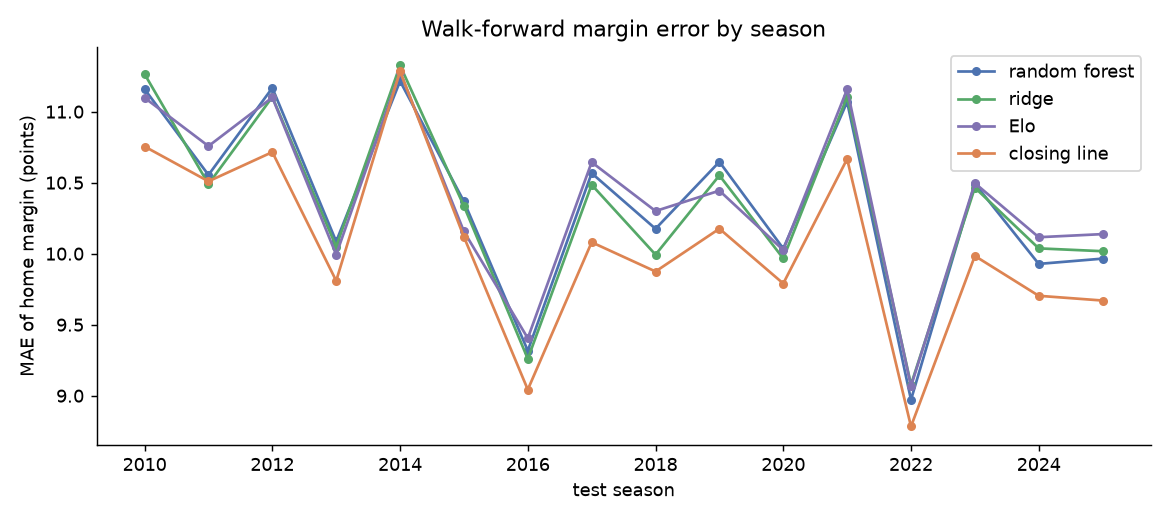
\includegraphics[width=0.95\textwidth]{rf_mae_by_season.png}
\caption{Margin error by test season. All methods share the hard and easy seasons; the closing line is lowest in 15 of 16.}
\label{fig:mae_season}
\end{figure}

\begin{figure}[H]
\centering
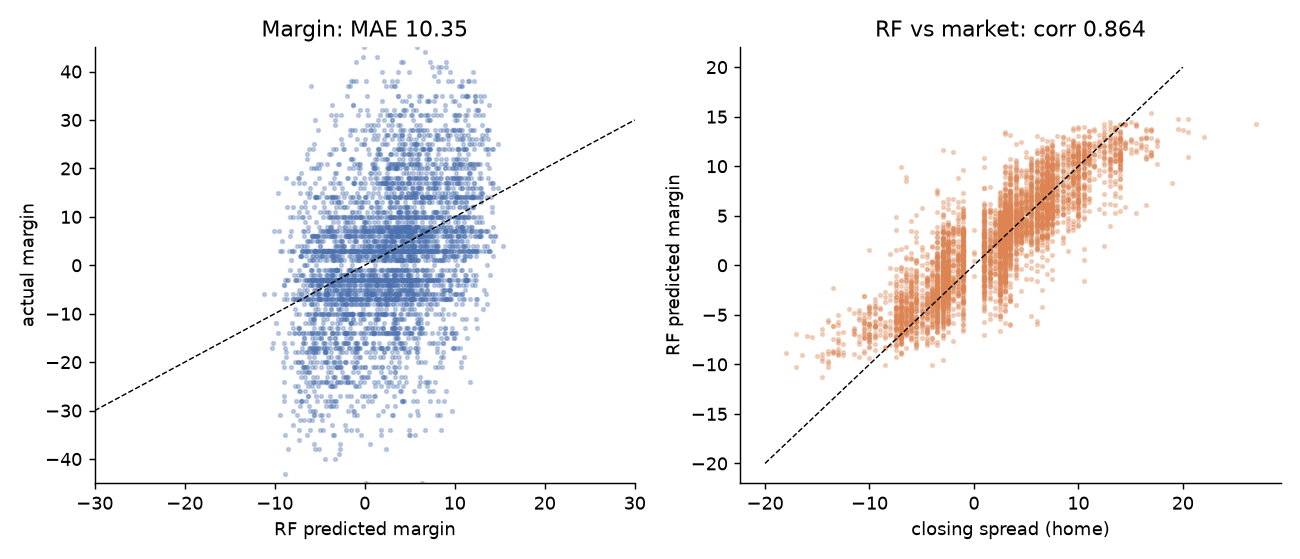
\includegraphics[width=0.95\textwidth]{rf_pred_vs_actual.png}
\caption{Left: predicted against actual margin. Right: the forest's margin against the closing spread (correlation 0.86).}
\label{fig:pred_actual}
\end{figure}

\subsection{The two-output structure}

Because the forest predicts a point in the $(h,a)$ plane, its residuals describe a two-dimensional distribution around that point (Table~\ref{tab:bivariate}, Figure~\ref{fig:bivariate}). The correlation between the home and away residuals is 0.01: once the two means are set, the leftover error in one score says nothing about the other. Residual spread grows with the predicted score, so high-scoring games are less predictable in points, as a Poisson-like scoring process implies. Calibration per score is good: when the forest predicts 20 points the team scores 20 on average, across the range 15 to 33.

\begin{table}[H]
\centering
\small
\begin{tabular}{lcc}
\toprule
\textbf{Quantity} & \textbf{Home} & \textbf{Away} \\
\midrule
Standard deviation of the actual score & 10.21 & 9.83 \\
Standard deviation of the residual & 9.64 & 9.36 \\
Range of predicted scores & 15.8 to 33.3 & 13.3 to 30.4 \\
Residual s.d., lowest third of predictions & 9.20 & 8.88 \\
Residual s.d., highest third of predictions & 10.11 & 9.76 \\
\bottomrule
\end{tabular}
\caption{Residual structure of the two-output forest, 4,363 out-of-sample games. Residual correlation 0.011.}
\label{tab:bivariate}
\end{table}

\begin{figure}[H]
\centering
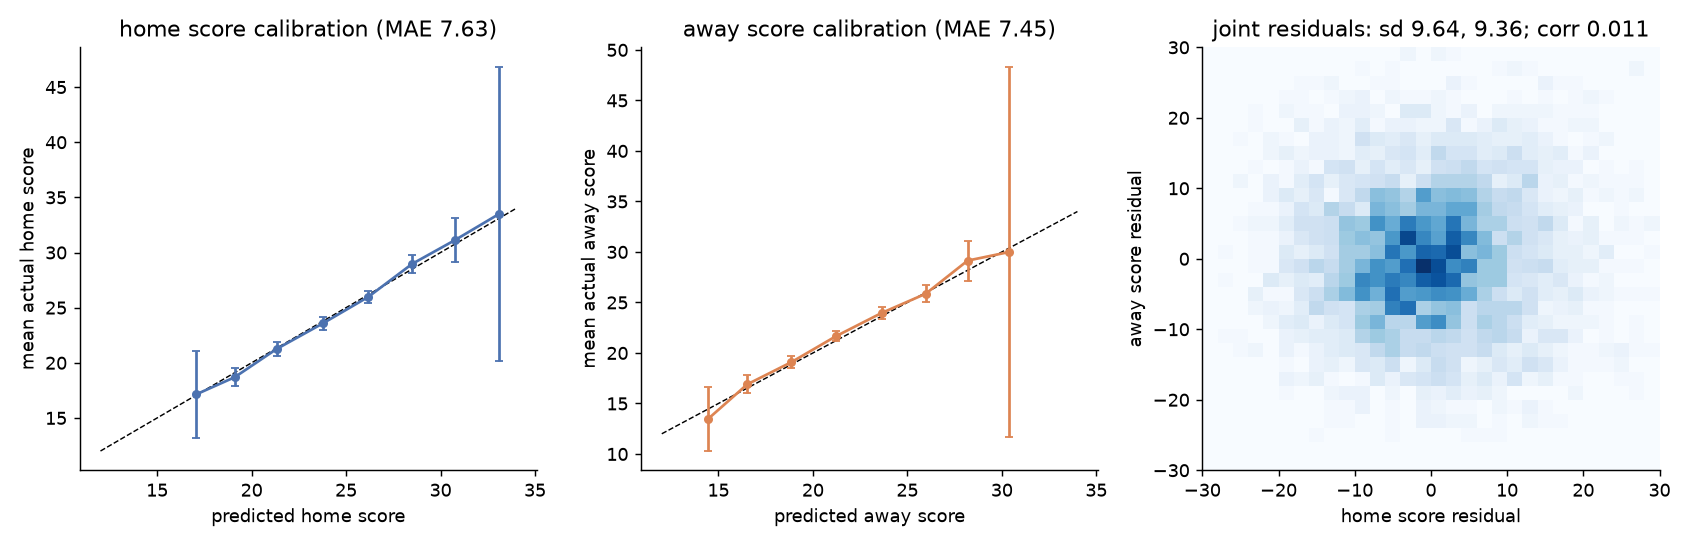
\includegraphics[width=0.98\textwidth]{rf_bivariate.png}
\caption{Calibration of the home and away score predictions and the joint distribution of the two residuals.}
\label{fig:bivariate}
\end{figure}

These residual statistics are the parameters $(\sigma_h,\sigma_a,\rho)$ of the probabilistic extension suggested by Professor Amine. Used as a pooled bivariate normal around the two predicted scores, they give a home-win probability with Brier score 0.2207 over 2016--2025, against 0.2220 for Elo and 0.2108 for the de-vigged moneyline; placing the two predicted means on the empirical grid of Section~\ref{sec:pricing} gives 0.2213. The probabilities are calibrated (Figure~\ref{fig:rf_cal}); the gap to the market is in sharpness, not bias.

\begin{figure}[H]
\centering
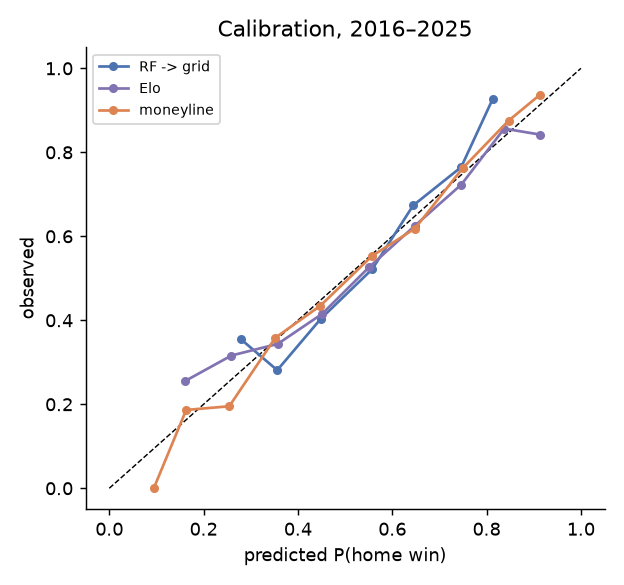
\includegraphics[width=0.5\textwidth]{rf_calibration.png}
\caption{Calibration of home-win probabilities, 2016--2025.}
\label{fig:rf_cal}
\end{figure}

\subsection{What the forest uses}

Averaged over the sixteen fits, the five most important features are all team-strength summaries from results: the difference in opponent-adjusted weighted margin, the difference in weighted margin, and the three Elo features (Figure~\ref{fig:importance}). The first play-by-play feature is yards per play, followed by the starting quarterback's success rate and EPA per dropback and points per drive. Injury, rest and weather features are far down the list. Most of what the model knows is how good each team has been; the efficiency and quarterback features refine that at the margin. The forest used all 759 features with no selection or tuning and matched a regularised linear model, which is what Professor Shasha expected.

\begin{figure}[H]
\centering
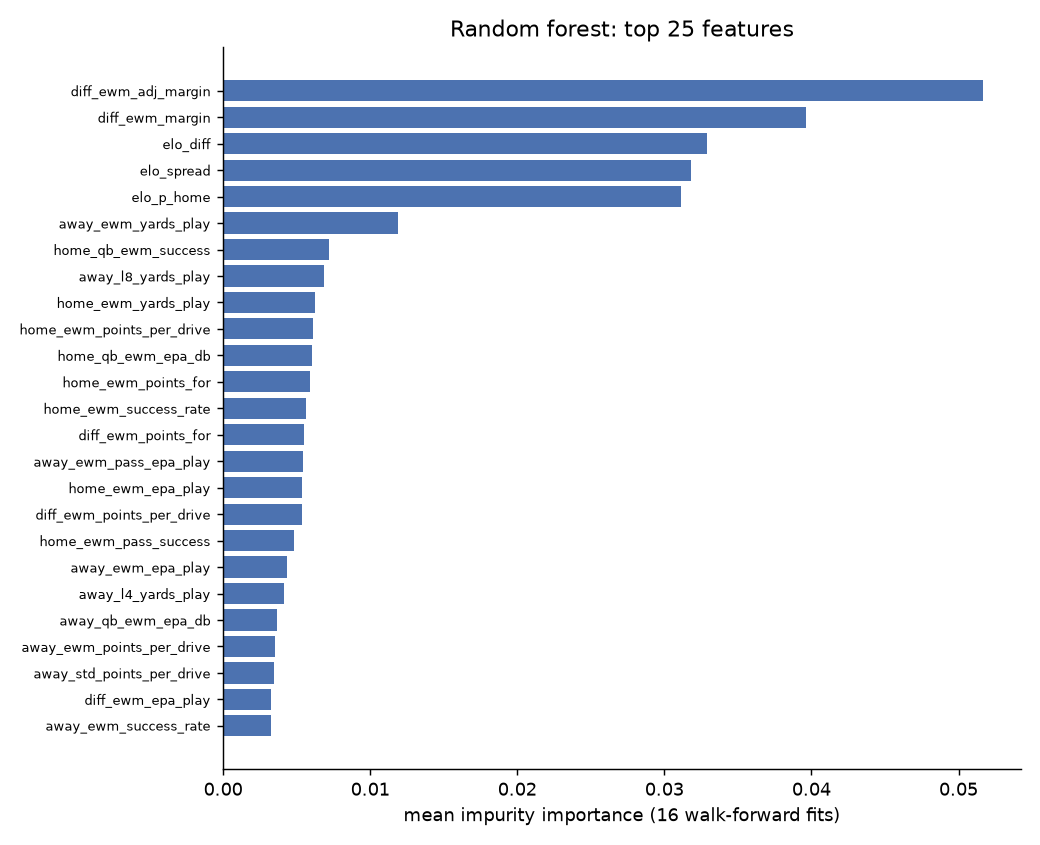
\includegraphics[width=0.75\textwidth]{rf_importance.png}
\caption{Top 25 features by mean impurity importance over the sixteen walk-forward fits.}
\label{fig:importance}
\end{figure}

\subsection{Can an ensemble do better?}

Professor Shasha asked whether an ensemble of the models we have, or can obtain, improves on them. We stacked by least squares, fitting weights on earlier seasons' out-of-sample predictions and applying them to the next season, 2013--2025. To our three models we added two public forecasts, nfelo~\cite{nfelo} (a public Elo variant with a quarterback adjustment; we use its rating difference before any regression toward the market) and FiveThirtyEight's Elo (available to 2020), and the sportsbook \emph{opening} line, which the nfelo files carry (Table~\ref{tab:ensemble}, Figure~\ref{fig:ensemble}).

\begin{table}[H]
\centering
\small
\begin{tabular}{lcp{6cm}}
\toprule
\textbf{Forecast} & \textbf{Margin MAE} & \textbf{Note} \\
\midrule
Random forest (ours) & 10.22 & \\
Ridge (ours) & 10.20 & \\
Elo (ours) & 10.25 & \\
Stack of our three & 10.18 & weights 0.19 / 0.36 / 0.51 \\
nfelo, pure model & 10.01 & history back-computed with the current model, so optimistic \\
Stack: ours + nfelo & 10.04 & our models receive weight near 0 \\
Opening line & 10.02 & \\
Closing line & 9.92 & \\
Stack: ours + nfelo + closing line & 9.95 & closing line 0.58, nfelo 0.72, ours near 0 \\
\bottomrule
\end{tabular}
\caption{Stacking test, home margin, 2013--2025 (3,562 games with all forecasts available).}
\label{tab:ensemble}
\end{table}

\begin{figure}[H]
\centering
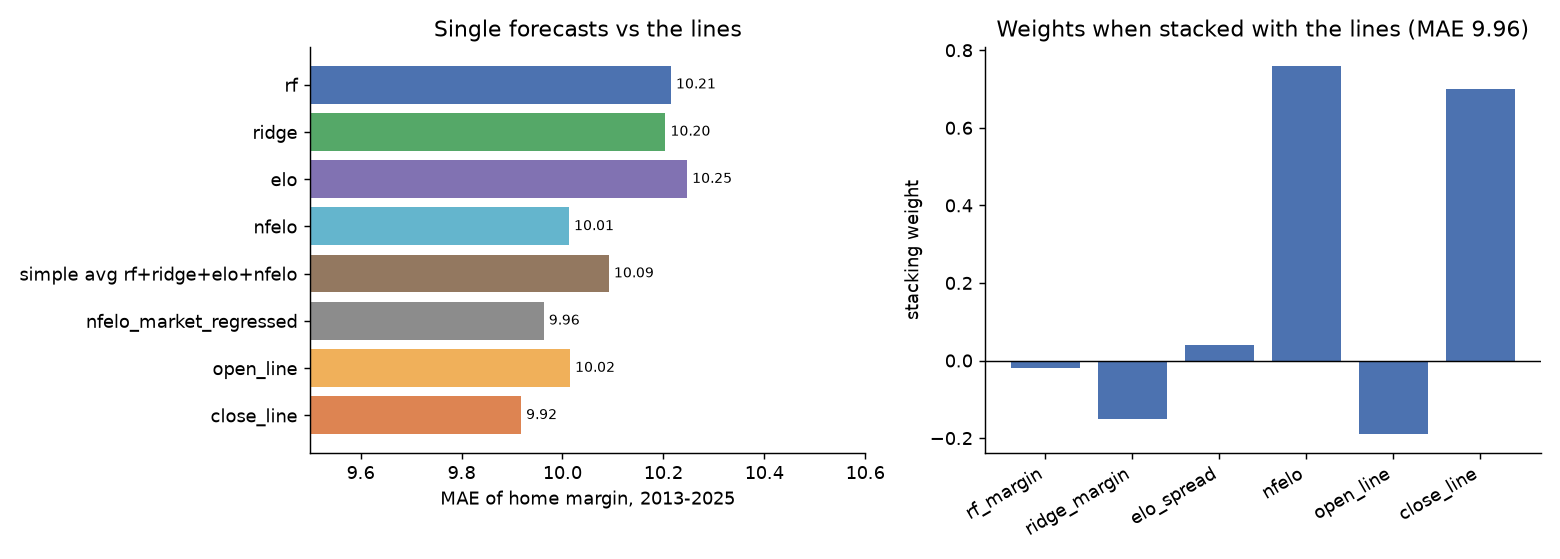
\includegraphics[width=0.98\textwidth]{ensemble_external.png}
\caption{Left: single forecasts and the lines. Right: stacking weights when our models, nfelo and both lines are combined.}
\label{fig:ensemble}
\end{figure}

Averaging our own models gains only a few hundredths of a point, because their predictions are correlated at 0.89--0.94. nfelo is a better single forecast than anything we built, by about 0.2 points, which we attribute to its quarterback adjustment and to its published history being generated by the current version of the model. Most important, no stack improves on the closing line: whenever the line is a component it takes nearly all the weight. The same holds for totals, where the opening total (10.47) is in fact slightly better than the closing total (10.53) in this sample. Ensembling what we have does not beat the market; an ensemble that could would need forecasts carrying information the market does not yet have.

\subsection{Full distributions and the Vegas lines}

The second question was whether the models can give a distribution for the margin and the total and how it compares with the lines. The two predicted scores set the centre, and the distribution around them comes either from the bivariate normal with the residual covariance or from the empirical grid tilted so that its mean margin and total match the forest (Figure~\ref{fig:gamedist}). From either, the probability of any outcome is a sum: $P(\text{home wins})$, $P(\text{home covers the spread})$, $P(\text{over the total})$.

\begin{figure}[H]
\centering
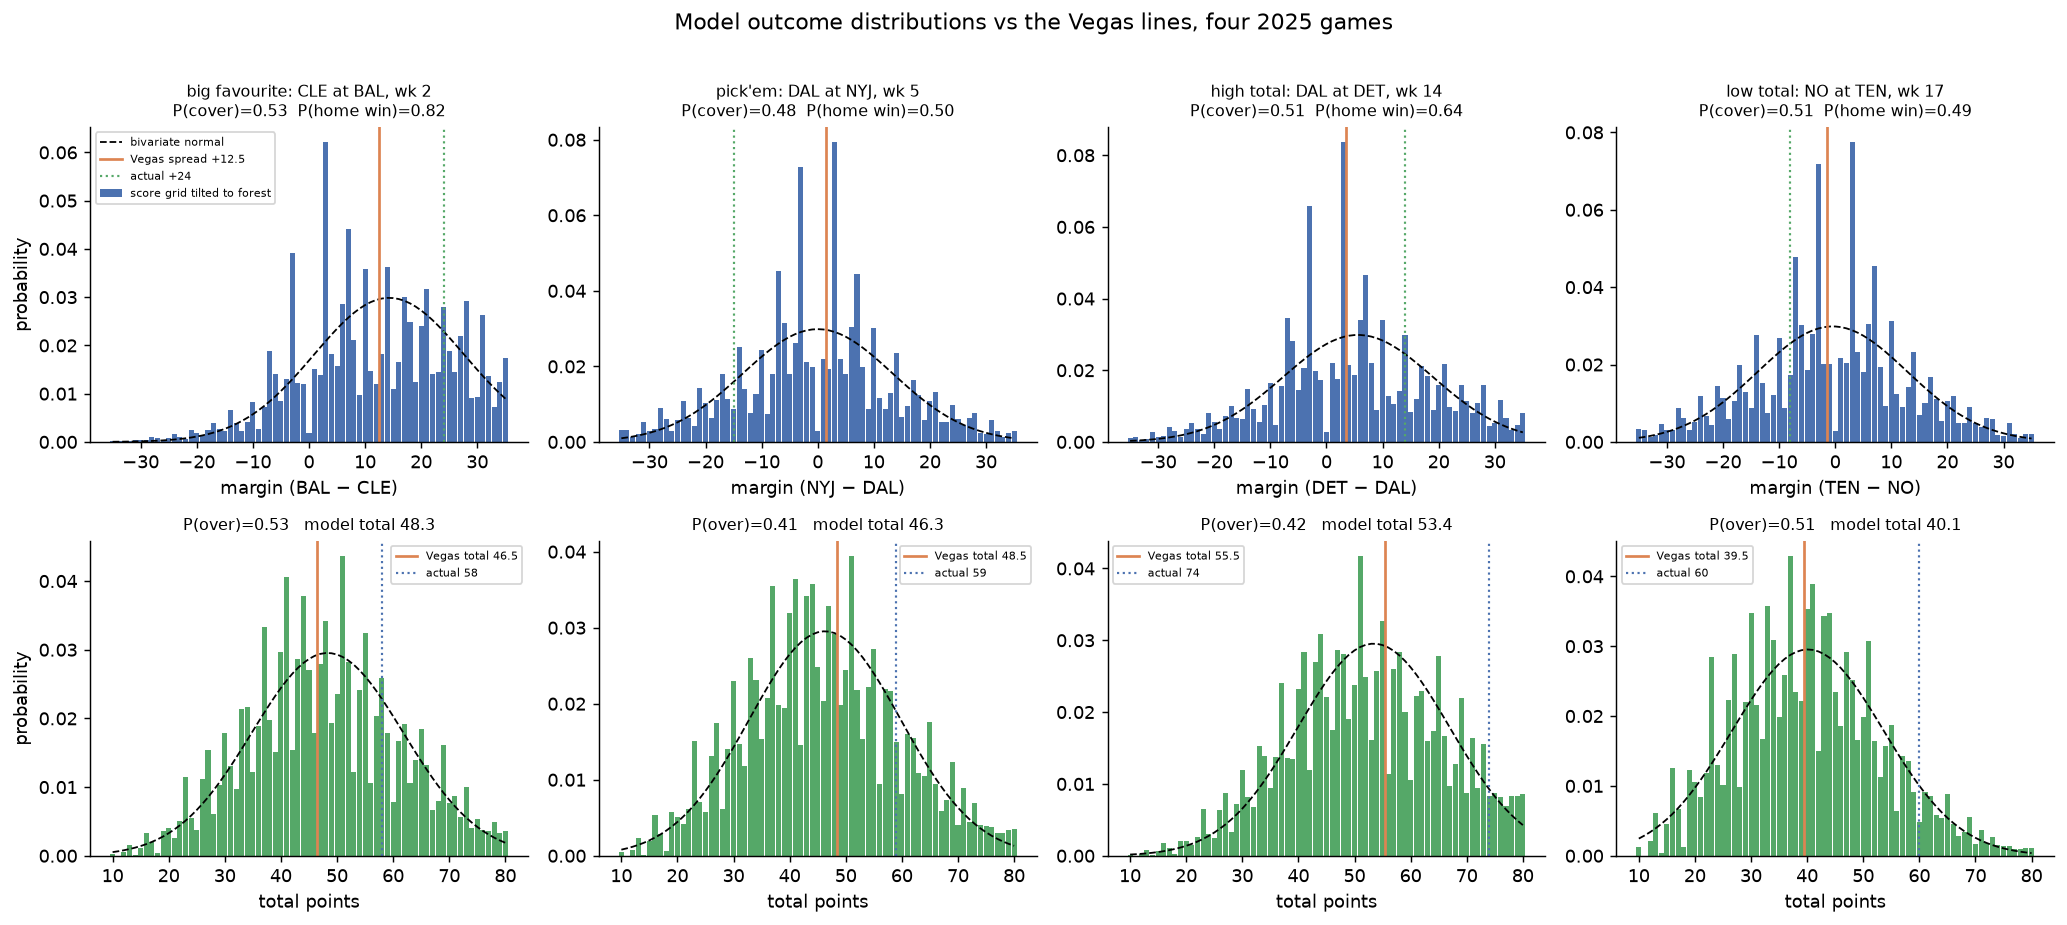
\includegraphics[width=\textwidth]{game_distributions.png}
\caption{Four 2025 games. Top: margin distribution from the tilted score grid (bars) and the bivariate normal (dashed), with the Vegas spread (orange) and the actual margin (dotted). Bottom: the same for the total.}
\label{fig:gamedist}
\end{figure}

Across all 2,758 games from 2016 to 2025, the model's $P(\text{cover})$ averages 0.50 with a standard deviation of 0.09 and $P(\text{over})$ averages 0.49 with a standard deviation of 0.08; only a quarter of games get a cover probability outside 0.40--0.60. The calibration of these probabilities against outcomes is flat (Figure~\ref{fig:coverover}): when the model says 65\% to cover, teams cover about 52\%. Brier scores of 0.257 for cover and 0.255 for over, against 0.25 for a coin, say the same thing. The distributions are internally consistent and calibrated for outcomes the market has not priced, but they do not know which side of the Vegas number will hit. This is the expected result for an efficient line, and it is the reason the engine's value lies in pricing the whole distribution consistently rather than in picking sides.

\begin{figure}[H]
\centering
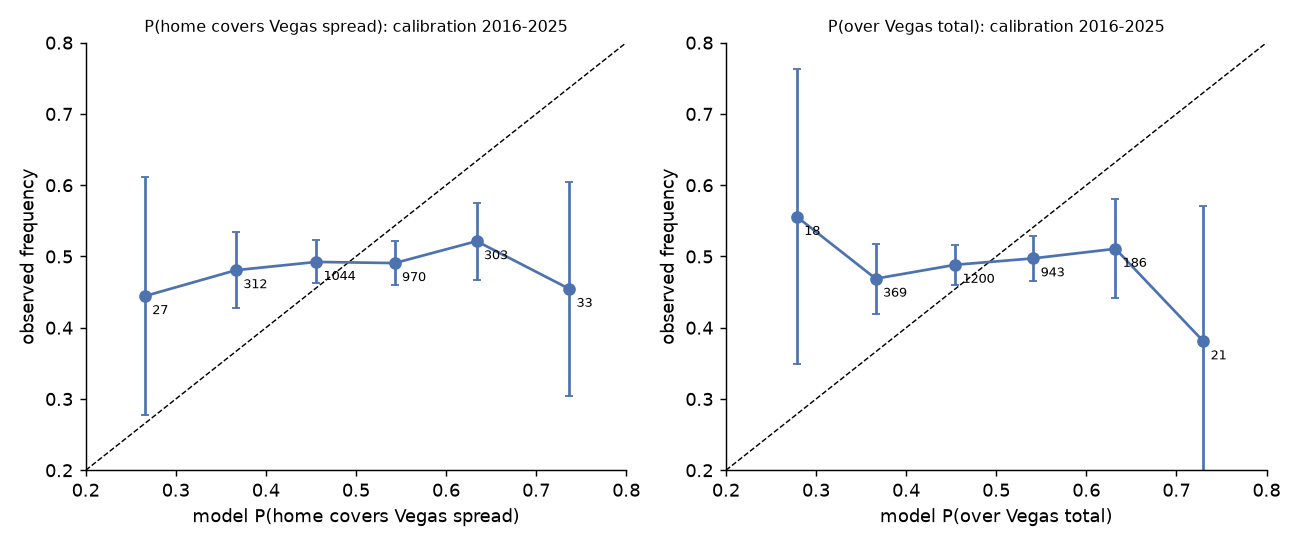
\includegraphics[width=0.95\textwidth]{cover_over_calibration.png}
\caption{Calibration of the model's cover and over probabilities, 2016--2025; bin sizes shown.}
\label{fig:coverover}
\end{figure}
